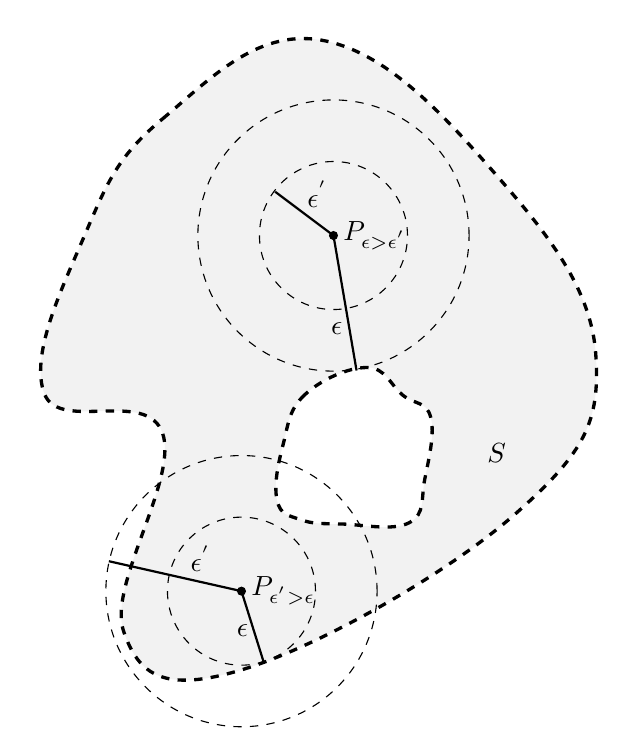
\begin{tikzpicture}

\draw [very thick,dashed,fill=gray!10] plot[smooth cycle, tension=.7] coordinates {(-4,4.5) (-3,6) (-1,7) (1.2182,5.305) (2.5,3) (1.5,1) (-2,-1) (-3.5,-0.5) (-3,2) (-4.5,2.5)};
\draw [very thick,dashed,fill=white]  plot[smooth cycle, tension=.7] coordinates {(-0.4047,2.84) (-1.1942,2.4963) (-1.4728,1.8555) (-1.5471,1.1497) (-1.2498,0.9082) (-0.7205,0.8525) (0.134,0.8711) (0.3289,1.4282) (0.4032,2.2084) (0.0503,2.487) };

\coordinate (S) at (1,2);
\node[{anchor=north west }] at (S){$S$};
\coordinate (N) at (-2,0) {};
\draw [black,dashed]  (N)circle (49pt);: 
\draw  [black,dashed](N) circle (0.94);
\draw[fill=black]  (N) circle (0.05);

\coordinate (N0) at (-1.7198,-0.8952) {} {};
\coordinate (N1) at (-3.6839,0.38) {} {} {} {};
\draw[ thick ]    plot[] coordinates { (N1)(N)  };
\draw[ thick ]    plot[] coordinates { (N0)(N)  };
\coordinate (T0) at (-2.1834,-0.7031) {} {} {} {} {};
\coordinate (T1) at (-2.2653,0.1265) {} {} {} {};
\node[{anchor=south west }] at (T0){$\epsilon$};
\node[{anchor=south east }] at (T1){$\epsilon^{'}$};
\node[right] at (N){$P_{\epsilon^{'}>\epsilon}$};


\coordinate (N2) at (-0.8317,4.5164) {} {};
\draw [black,dashed]  (N2)circle (49pt);: 
\draw  [black,dashed](N2) circle (0.94);

\coordinate (N20) at (-0.5385,2.802) {} {} {};
\coordinate (N21) at (-1.5724,5.0726) {} {} {};
\draw[ thick ]    plot[] coordinates { (N21)(N2)  };
\draw[ thick ]    plot[] coordinates { (N20)(N2)  };
\coordinate (T20) at (-0.9864,3.1348) {} {} {} {} {};
\coordinate (T21) at (-0.7827,4.7518) {} {} {};
\node[{anchor=south west }] at (T20){$\epsilon$};
\node[{anchor=south east }] at (T21){$\epsilon^{'}$};
\node[right] at (N2){$P_{\epsilon>\epsilon^{'}}$};;
\draw[fill=black]  (N2) circle (0.05);
\end{tikzpicture}